\documentclass[journal]{IEEEtran}
\usepackage{cite}
\usepackage{amsmath}
\usepackage{booktabs}
\usepackage{graphicx}
\usepackage{tikz}
\usetikzlibrary{arrows.meta,positioning,fit,backgrounds}
\usepackage{algorithm}
\usepackage{algpseudocode}
\usepackage{amsthm}
\usepackage[hidelinks]{hyperref}

\newtheorem{proposition}{Proposition}

\begin{document}

\title{GridSense: Measuring the Carbon, Capacity, and Forecast-Robustness\\Value of Coordinated Residential EV Charging}

\markboth{GridSense: Coordinated Residential EV Charging}{Sahoo \MakeLowercase{\textit{ et al.}}: Carbon, Capacity, and Forecast-Robustness Value of Coordinated EV Charging}

\author{
\begin{tabular}[t]{@{}c@{\hspace{1.2cm}}c@{}}
\begin{tabular}[t]{@{}c@{}}
Aditya Ayushman Sahoo\\
Department of Computational Intelligence,\\
School of Computing,\\
SRM Institute of Science and Technology,\\
Kattankulathur -- 603203\\
adityaasahoo@gmail.com
\end{tabular}
&
\begin{tabular}[t]{@{}c@{}}
Himanshi Mohapatra\\
B.Tech, Computer Science,\\
~\\
Siksha `O' Anusandhan University,\\
Bhubaneswar -- 751030\\
mohapatrahimanshi@gmail.com
\end{tabular}
\end{tabular}
\thanks{Code, measured data, and the scripts that regenerate every figure and table in this paper are maintained in the project repository; see its README for reproduction instructions.}}

\maketitle

\begin{abstract}
Uncoordinated residential electric-vehicle (EV) charging concentrates load at the moment drivers arrive home, which already sits close to a distribution grid's daily peak. This paper reports a measurement-driven study of what a linear-programming (LP) charge scheduler is actually worth, built and repeatedly corrected against real grid data rather than synthetic curves. We show the optimizer departs from a greedy, per-vehicle heuristic only once a coupling constraint -- a shared feeder limit or a peak-minimizing objective -- links vehicles together; absent one, heterogeneity in arrival time, energy need, and charger rating does not by itself make optimization necessary. A backtest against a corrected four-year Spanish grid record shows the carbon saving from coordinated charging is real but small and long-tailed (median 2.0\%, fleet total 6.6\%), and that an early synthetic carbon-intensity curve used in this project scored \emph{negative} once measured against truth, which motivates the measurement-first approach used throughout. The larger result is capacity: coordinating a street's charging raises a 250~kW distribution transformer's EV hosting capacity by a median 4.1$\times$ (bootstrap 95\% CI [3.73$\times$, 4.24$\times$]), a result validated against real UK and Spanish smart-meter panels. Extending the model to India's two- and three-wheeler-dominated fleet shows the capacity gain transfers (3.5$\times$) but the carbon mechanism collapses (overnight saving 0.09\%, 22$\times$ smaller than Spain's, on a grid 2.3$\times$ dirtier). We then price what a real distribution company gives up by not having a perfect forecast of neighbouring demand: a CI-backed search over feeder margins finds a 5\% overload-reliability target out of reach everywhere on an 11-point, bootstrap-confirmed grid (best case 25.0\%, 95\% CI [17\%, 34\%], more than 3$\times$ the target), and re-forecasting hourly instead of committing once to a day-ahead margin makes the overload risk worse in most cells, not better, by a mean 15.0 percentage points.
\end{abstract}

\begin{IEEEkeywords}
carbon-aware scheduling, demand response, distribution transformer hosting capacity, electric vehicle charging, forecast uncertainty, linear programming, model predictive control, residential load management, smart grid, vehicle-to-grid
\end{IEEEkeywords}

\section{Introduction}

Residential electric-vehicle charging is, by default, synchronized with the worst possible hour to add load: a driver arrives home in the early evening and plugs in immediately, at precisely the moment a distribution feeder is already carrying its own residential peak. As EV adoption rises, this habit is the mechanism by which charging threatens both carbon intensity, because evening hours often lean on the grid's most carbon-intensive dispatchable generation, and distribution capacity, because a street transformer sized for houses alone was never meant to also carry a fleet of chargers at the one hour everyone wants power at once.

Scheduling charging against something other than arrival time -- grid carbon intensity, price, or a transformer's rating -- is a well-studied idea. What is less common is a sustained, adversarial measurement of what that scheduling is actually worth once naive assumptions are replaced with measured grid data, and once every headline number is checked against what a real operator -- without perfect foresight -- could actually achieve. This paper reports that measurement exercise for GridSense, a full-stack EV charge-scheduling system whose linear-programming (LP) core, hosting-capacity analysis, and forecast-robustness results have each been built, found wrong at least once, corrected, and re-measured. We treat the corrections as part of the result rather than hiding them, because several materially changed the answer: an early version of the headline hosting-capacity gain was inflated 2.7$\times$ by an unstaggered fleet, a residential baseline load was overstated sevenfold, and a synthetic carbon-intensity curve used in early development turned out to be phase-inverted relative to the real grid and scored worse than no scheduling at all.

\subsection{Contributions}
\begin{itemize}
  \item \textbf{A coupling-constraint characterization of when optimization matters.} We show formally and empirically that an LP scheduler without a constraint linking vehicles is \emph{separable} -- a ten-line greedy loop reproduces it to within numerical tolerance -- and that vehicle heterogeneity alone does not change this. Only a shared feeder limit or a peak-minimizing objective makes coordination a genuine optimization problem.
  \item \textbf{A corrected, long-horizon carbon-saving backtest.} Replaying the scheduler over 1,448 nights of a corrected Spanish grid record shows a median nightly saving of 2.0\% and a fleet-wide total of 6.6\% -- real, but an order of magnitude below what a smooth synthetic carbon curve suggests, and concentrated in a long right tail rather than uniform across nights.
  \item \textbf{A validated hosting-capacity result with a formal confidence interval.} Coordinating a 200-home street's EV charging against a 250~kW transformer raises its hosting capacity by a median 4.1$\times$ (bootstrap 95\% CI [3.73$\times$, 4.24$\times$], not just the 3.3--5.3$\times$ full range across fleet draws); the result is checked against real smart-meter panels from Spain and the UK and against a published figure for India, and three distinct modeling errors that previously inflated it are documented and corrected.
  \item \textbf{A forecast-robustness study with two negative results.} A day-ahead ridge forecaster captures 68.9--80.9\% of the achievable carbon saving depending on grid era, and a decision threshold (``forecast gate'') that defers to arrival-time charging on low-confidence nights removes most of the harm a forecast can otherwise do. Separately, rebuilding the scheduler as a rolling-horizon (MPC-style) controller that re-solves every hour \emph{loses} to the one-shot day-ahead plan, and a deferral penalty meant to fix this makes it monotonically worse.
  \item \textbf{A transfer to India's EV mix, and a new robustness result for it.} India's fleet is 91\% two- and three-wheelers, not cars; re-deriving every input for that mix shows the hosting-capacity mechanism transfers (3.5$\times$) while the carbon-saving mechanism does not (overnight saving 0.09\%). We then show, with a bootstrap-CI-backed search over an 11-point margin grid, that no feeder margin reaches a 5\% overload-reliability target under realistic forecast error (best case 25.0\%, 95\% CI [17\%, 34\%]), and that re-forecasting every hour instead of committing once to a day-ahead margin makes the overload risk \emph{worse} in most tested cells -- the same loss mechanism found for carbon-aware MPC, now demonstrated on a capacity-reliability problem.
\end{itemize}

The rest of this paper is organized as follows. Section~\ref{sec:related} positions this work against the demand-response, hosting-capacity, and forecast-driven-control literature. Section~\ref{sec:method} formalizes the scheduler, the hosting-capacity search, and the two robustness controllers. Section~\ref{sec:experiments} reports results. Section~\ref{sec:discussion} discusses what the measurements imply, Section~\ref{sec:limitations} states what remains open, and Section~\ref{sec:conclusion} concludes.

\section{Related Work and Positioning}
\label{sec:related}

The idea that EV charging should respond to something other than arrival time is well established; what this paper adds is a sustained measurement of that idea's value against real, cross-validated grid data, including the forecast error and control-timing effects that separate a scheduler's achievable value from what it can actually realize. Table~\ref{tab:positioning} summarizes the gap this paper targets against each area below.

\begin{table*}[t]
\centering
\caption{Positioning against prior work.}
\label{tab:positioning}
\begin{tabular}{p{2.6cm}p{4.3cm}p{5.0cm}p{4.6cm}}
\toprule
\textbf{Prior area} & \textbf{Representative work} & \textbf{What it does} & \textbf{What this paper adds} \\
\midrule
Coordinated EV charging / demand response & Kakkar et al.~\cite{kakkar2024} & Taxonomy of EV demand-response schemes: forecasting, optimization, security & A single system measured end-to-end on real grid data, with the optimizer's own necessity condition proven \\
Transformer-level hosting capacity & Golgol et al.~\cite{golgol2024}; Paudyal et al.~\cite{paudyal2021} & Feeder/transformer-level hosting-capacity tools on AMI or synthetic feeders & A capacity result cross-checked against real smart-meter panels in two countries, and against a second national EV mix (India) \\
Forecast-driven / MPC scheduling & Yang et al.~\cite{yang2020bmpc}; Lago et al.~\cite{lago2021}; Uniejewski~\cite{uniejewski2024} & Rolling-horizon and regularized-forecast methods for deferrable loads and prices & A head-to-head one-shot-vs-rolling comparison that finds rolling control \emph{loses}, on two different objectives (carbon, capacity reliability) \\
Vehicle-to-grid economics & Gandhi and White~\cite{gandhi2021v2g} & City-scale V2G profitability as a function of battery performance & A V2G result decomposed by objective (carbon, cost, peak) with an explicit abatement-cost-per-kg comparison to a carbon-market price \\
Carbon-aware load shifting & Radovanovi{\'c} et al.~\cite{radovanovic2021}; WattTime~\cite{watttime_moer} & Carbon-aware compute scheduling; marginal-vs-average emissions signals & The average/marginal distinction applied to residential EV charging, with the gap between the two signals measured rather than assumed \\
\bottomrule
\end{tabular}
\end{table*}

\subsection{Coordinated and demand-responsive EV charging}
Kakkar et al.\ survey EV demand-response schemes across load forecasting, optimization, and security, and organize the field around a device-to-grid taxonomy~\cite{kakkar2024}. That and related surveys establish \emph{that} coordination is useful; they do not, in general, isolate \emph{when} an optimizer is doing something a much simpler heuristic could not. GridSense's coupling-constraint result (Section~\ref{sec:method}) answers that question directly for an LP formulation with energy, power, and window constraints: coordination only earns its keep once vehicles are linked by a shared limit or a peak objective. This paper's gap relative to this literature is a necessity condition for optimization, stated and tested rather than assumed.

\subsection{Distribution-level hosting capacity under EV load}
Golgol et al.\ study residential EV charging's effect on feeder transformers in Arizona using measured advanced-metering data and propose a coordinated-charging algorithm with a per-transformer confidence-level cap~\cite{golgol2024}. Paudyal et al.\ describe an NREL tool that evaluates thermal, voltage, and transformer-loading limits on a set of real feeder models, including extreme fast-charging scenarios~\cite{paudyal2021}. Both works are feeder-specific case studies; neither cross-validates a capacity-gain figure against independently measured household-load panels in more than one country, and neither extends the analysis to a non-Western vehicle mix. This paper's hosting-capacity result is validated against two real smart-meter panels (Section~\ref{sec:experiments}) and re-derived for India's two- and three-wheeler-dominated fleet, which is the gap addressed here.

\subsection{Forecast-driven and predictive scheduling under uncertainty}
Yang et al.\ formulate deferrable-load scheduling under demand charges as a block model-predictive control problem and note that setting an appropriate terminal cost becomes difficult once the demand forecast carries real error~\cite{yang2020bmpc} -- precisely the difficulty this paper's rolling-horizon result (Section~\ref{sec:experiments}) encounters and measures rather than assumes away. Lago et al.\ benchmark day-ahead price-forecasting algorithms and establish regularized linear models as a durable baseline~\cite{lago2021}; Uniejewski compares regularization penalties for the same task and situates ridge regression as the historically first choice~\cite{uniejewski2024}. GridSense's deployed forecaster is exactly such a ridge model, chosen because it is deployable without a machine-learning runtime dependency, and the gap this paper targets is not a better forecaster but an honest accounting of what a given forecaster's error does to a committed decision -- both hour-by-hour (Section~\ref{sec:experiments}F) and under a binary act/defer gate (Section~\ref{sec:experiments}E).

\subsection{Vehicle-to-grid economics}
Gandhi and White model city-scale vehicle-to-grid (V2G) economics and find that how fast a vehicle charges and how much energy it loses round-tripping through the battery matter more to an owner's profit than price volatility does, in every city they model~\cite{gandhi2021v2g}. That work treats V2G as a standalone revenue question; this paper instead decomposes V2G's effect by scheduling objective (carbon, cost, peak) and converts the carbon result into an explicit abatement cost per kilogram, comparable to a carbon-market price, which is the gap addressed in Section~\ref{sec:experiments}.

\subsection{Carbon-aware and marginal-vs-average load shifting}
Radovanovi{\'c} et al.\ describe Google's carbon-intelligent compute platform, which shifts flexible datacenter workload using day-ahead carbon forecasts~\cite{radovanovic2021}. WattTime's marginal operating emissions rate (MOER) methodology argues that load-shifting decisions should respond to the \emph{marginal}, not average, generator~\cite{watttime_moer}. GridSense schedules against an average-intensity signal built from measured generation mix and IPCC lifecycle factors, and explicitly measures -- rather than assumes -- how far that average signal diverges from an estimated marginal one (Section~\ref{sec:experiments}). The gap here is empirical: quantifying the average/marginal gap for a real residential-charging decision, rather than arguing from the concept alone.

\medskip
Across all five areas, the common gap this paper fills is the same: prior work typically reports an optimizer's \emph{achievable} value under an assumption (perfect information, a synthetic load shape, an idealized battery), while this paper repeatedly re-measures that value once the assumption is replaced with real data or a forecast's real error, and reports the cases -- the inverted synthetic carbon curve, the rolling-horizon loss, the intraday-correction loss -- where doing so overturns the naive answer.

\section{System and Method}
\label{sec:method}

\subsection{Scheduling problem}
GridSense schedules a fleet of vehicles $v \in V$ over a 24-hour horizon $h \in \{0,\dots,23\}$. Each vehicle has an energy requirement $E_v$ (kWh), a charger power rating $P_v$ (kW), an arrival hour $a_v$, and a deadline hour $b_v$ (with overnight wraparound when $b_v \le a_v$), giving an availability window
\begin{equation}
\mathcal{H}_v = \{a_v, a_v{+}1, \dots, 23, 0, \dots, b_v{-}1\} \quad \text{(or } [a_v,b_v) \text{ if } b_v>a_v\text{).}
\label{eq:window}
\end{equation}
Charging and discharging are modeled as separate non-negative variables $c_{v,h}, d_{v,h} \ge 0$ rather than one signed variable, because round-trip efficiency $\eta$ applies only to the discharge leg; the net grid draw is $x_{v,h} = c_{v,h} - d_{v,h}$. Outside $\mathcal{H}_v$ both variables are fixed to zero, and $c_{v,h}\le P_v$, $d_{v,h}\le D_v$ (0 unless vehicle-to-grid is enabled). The energy constraint, net of discharge losses, is
\begin{equation}
\sum_{h=0}^{23} \big(c_{v,h} - d_{v,h}\,\kappa\big) = E_v, \qquad \kappa = 1/\eta,
\label{eq:energy}
\end{equation}
with $\eta = 0.90$ throughout. When V2G is enabled, the pack's state of charge is tracked along the plug-in window in window order (not clock order, since the window crosses midnight):
\begin{equation}
S_{v,i} = S_{v,i-1} + c_{v,h_i} - d_{v,h_i}\,\kappa, \qquad r_v \le S_{v,i} \le \beta_v,
\label{eq:soc}
\end{equation}
for the $i$-th hour $h_i$ of $\mathcal{H}_v$, with reserve floor $r_v$ and pack size $\beta_v$, and an optional cap $\sum_i d_{v,h_i} \le \Delta_v$ standing in for battery-wear cost the model does not otherwise price.

Three objectives are supported. Minimizing emissions or cost is linear in carbon intensity $g_h$ or price $p_h$:
\begin{equation}
\min \sum_{v,h} x_{v,h}\, g_h \qquad \text{or} \qquad \min \sum_{v,h} x_{v,h}\, p_h .
\label{eq:obj-linear}
\end{equation}
Minimizing peak introduces an auxiliary variable $\pi$ against the residential baseline $L_h$:
\begin{equation}
\min \pi \quad \text{s.t.}\quad \pi \ge \sum_v x_{v,h} + L_h \ \ \forall h.
\label{eq:obj-peak}
\end{equation}
An optional shared feeder limit $F$ constrains every hour:
\begin{equation}
\sum_v x_{v,h} + L_h \le F \qquad \forall h.
\label{eq:feeder}
\end{equation}
The problem is solved with PuLP's bundled CBC solver.

\subsection{The coupling-constraint condition}
\label{sec:coupling}
\begin{proposition}
If no constraint links vehicles -- i.e.\ neither \eqref{eq:obj-peak} nor \eqref{eq:feeder} is active -- the problem \eqref{eq:energy}--\eqref{eq:obj-linear} is separable: its optimum is achieved by each vehicle independently filling its own cheapest hours in $\mathcal{H}_v$, which a greedy per-vehicle loop computes directly.
\end{proposition}
\begin{proof}[Proof sketch]
With neither \eqref{eq:obj-peak} nor \eqref{eq:feeder} active, the objective $\sum_{v,h} x_{v,h}g_h$ and the constraint set both decompose across $v$: \eqref{eq:energy} and the box bound $0 \le c_{v,h} \le P_v$ (zero outside $\mathcal{H}_v$) involve only vehicle $v$'s own variables. The joint LP is therefore exactly $|V|$ independent single-vehicle LPs, each minimizing $\sum_h c_{v,h}g_h$ subject to $\sum_h c_{v,h} = E_v$ and $0 \le c_{v,h} \le P_v$ -- a fractional knapsack. Its optimum is reached by filling hours of $\mathcal{H}_v$ in ascending order of $g_h$ until $E_v$ is met: if any feasible solution leaves spare capacity at a cheaper hour while drawing at a more expensive one, moving load from the latter to the former cannot raise the objective, by a standard exchange argument. That is exactly what the greedy loop computes.
\end{proof}
This holds regardless of heterogeneity in $a_v$, $b_v$, $E_v$, or $P_v$, because \eqref{eq:energy} and the window bound on $c_{v,h}$ involve only vehicle $v$'s own variables once the objective decomposes across $v$. Only \eqref{eq:obj-peak} (through the shared $\pi$) or \eqref{eq:feeder} (through the shared per-hour sum) couples vehicles together. A consequence is complexity, not just equivalence: sorting each vehicle's $|\mathcal{H}_v|$ hours by $g_h$ and filling them greedily costs $O\!\big(\sum_v |\mathcal{H}_v|\log|\mathcal{H}_v|\big)$, against a general-purpose LP solve over all $v,h$ jointly once a coupling constraint forces the problem back together. Section~\ref{sec:experiments}B measures the resulting LP-vs-greedy gap directly.

\subsection{Hosting-capacity search}
Hosting capacity is the largest fleet size $N$ a transformer rated $F$ can serve without breaching its limit, under (i) every vehicle charging the instant it arrives (``on arrival'') and (ii) the coordinated LP schedule. Algorithm~\ref{alg:hosting} finds it by bisection, bounded above by the energy-feasibility bound of Section~\ref{sec:method}C so the search can never mistake its own upper bound for a ceiling -- an error present in an earlier version of this analysis.
\begin{algorithm}[t]
\caption{Hosting-capacity bisection search}
\label{alg:hosting}
\begin{algorithmic}[1]
\Require fleet template $T$, baseline load $L$, feeder rating $F$
\Ensure maximum vehicle count $N^\star$ that does not breach $F$
\State $\mathit{hi} \gets$ energy-feasibility bound (Section~\ref{sec:method}C)
\State $\mathit{lo} \gets 0$
\While{$\mathit{hi} - \mathit{lo} > 1$}
  \State $\mathit{mid} \gets \lfloor (\mathit{lo}+\mathit{hi})/2 \rfloor$
  \State fleet $\gets$ instantiate($T$, $\mathit{mid}$ vehicles)
  \If{schedule(fleet, $L$, $F$) is feasible}
    \State $\mathit{lo} \gets \mathit{mid}$
  \Else
    \State $\mathit{hi} \gets \mathit{mid}$
  \EndIf
\EndWhile
\State \Return $\mathit{lo}$
\end{algorithmic}
\end{algorithm}
Published figures are the median of $N^\star$ over 20 draws of a realistic, staggered fleet (Section~\ref{sec:experiments}D), since a single draw was found to be unrepresentative (Section~\ref{sec:discussion}).

\subsection{Rolling-horizon and intraday-correcting controllers}
Two robustness controllers rebuild the one-shot scheduler to act under a day-ahead forecast rather than perfect information.

\textbf{Carbon MPC.} A ridge forecaster is trained per horizon $k=1,\dots,13$ hours ahead. At each hour the controller re-solves the one-shot LP against the current forecast and commits only the next hour, replaying over held-out nights.

\textbf{Intraday hosting-capacity controller.} For the capacity-reliability problem, the baseline $L$ is corrupted by a persistent AR(1) error process evaluated at each position $i$ of the charging window,
\begin{equation}
e_i = \rho\, e_{i-1} + \mathcal{N}\!\big(0,\ \sigma\sqrt{1-\rho^2}\big), \qquad \rho = 0.7,
\label{eq:ar1}
\end{equation}
chained in \emph{window} order so the chain correctly crosses midnight, with the forecast baseline $\hat L_h = L_h(1+e_i)$. A \emph{static} controller observes $e_0$ once at 18:00, commits a full-night schedule against $\hat L$ with a feeder margin $m$ (i.e.\ a cap of $(1-m)F$), and is scored against the true $L$. A \emph{rolling} controller instead re-forecasts every hour: at position $i$ it corrects the forecast for every remaining position $j \ge i$ toward zero bias, $\widehat{e}_j = \rho^{\,j-i+1}\, e_{i-1}$, and re-solves for only the vehicles not yet fully charged. Algorithm~\ref{alg:rolling} gives the per-draw procedure; $\textsc{SolveStep}$ is a local per-vehicle-group LP minimizing peak load, needed because the project's shared scheduler returns only a fleet's \emph{summed} hourly load, which cannot be credited back to individual groups in a stateful rolling loop (Section~\ref{sec:discussion}).
\begin{algorithm}[t]
\caption{Rolling intraday hosting-capacity controller (one draw)}
\label{alg:rolling}
\begin{algorithmic}[1]
\Require vehicle groups $G$ (aggregated by charger, arrival, deadline), true baseline $L$, cap $(1-m)F$, error draw $e$
\Ensure overload indicator for this draw
\State $\mathit{remaining}[g] \gets E_g$ for all $g \in G$
\For{$i \gets 0$ \textbf{to} $12$} \Comment{window positions, 18:00--06:00}
  \State $h \gets$ clock hour at position $i$
  \State reopen groups not yet arrived at position $i$
  \State $\hat L \gets$ true $L$ for positions $< i$; AR(1)-corrected forecast \eqref{eq:ar1} for positions $\ge i$
  \State $x \gets \textsc{SolveStep}(\{g : \mathit{remaining}[g]>0\}, \hat L, (1-m)F)$
  \For{$g \in G$}
    \State $\mathit{credit} \gets \min(x[g][h],\, \mathit{remaining}[g])$
    \State $\mathit{remaining}[g] \gets \mathit{remaining}[g] - \mathit{credit}$
  \EndFor
\EndFor
\State \Return $\big[\max_h (\text{committed load}_h + L_h) > F\big]$
\end{algorithmic}
\end{algorithm}
As a correctness check, both controllers must reproduce the static one-shot optimum exactly when $\sigma=0$ -- the same time-consistency property the project's test suite already pins for the carbon-objective scheduler. Two implementation defects were caught exactly this way before being trusted on noisy data (Section~\ref{sec:discussion}).

\subsection{Data sources}
\label{sec:data}
Table~\ref{tab:data} lists the measured sources behind every result in Section~\ref{sec:experiments}. Carbon intensity is derived from measured generation mix weighted by IPCC AR5 Annex~III lifecycle emission factors~\cite{ipcc2014ar5}, so Spanish, German, and Indian intensities are comparable by construction. Spain's day-ahead price uses the regulated PVPC tariff structure~\cite{ree_pvpc}. Residential baselines for the validation experiments (Section~\ref{sec:experiments}D) are built from real smart-meter panels: GoiEner for Spain~\cite{quesada2024goiener} and the refactored Low Carbon London panel for the UK~\cite{tindemans2023lcl}. India's EV mix is taken from national retail-registration statistics~\cite{fada2025}, and the illustrative time-of-day price used in the India simulator scenario follows the rebate structure reported for Maharashtra's distribution tariff~\cite{ceew2025tariff,merc2025}, labeled as an assumption rather than a measurement throughout.

\begin{table}[t]
\centering
\caption{Measured data sources.}
\label{tab:data}
\begin{tabular}{p{1.7cm}p{6.1cm}}
\toprule
\textbf{Series} & \textbf{Source} \\
\midrule
Spain generation mix, price (2015--2018, corrected) & Energy-Charts republication of ENTSO-E, cross-checked against Spain's grid operator (REE) \\
Spain generation mix, price (2025 era) & Energy-Charts day-ahead solar/wind/load/price series \\
Germany generation mix & Energy-Charts, 2023--2026 \\
India generation mix & Grid-India Daily PSP Report, 15-minute, 555 days \\
Lifecycle emission factors & IPCC AR5 WG3 Annex~III~\cite{ipcc2014ar5} \\
Residential baseline (Spain, modeled) & ENTSO-E system load, scaled to IDAE's household consumption figure \\
Residential baseline (Spain, validated) & GoiEner smart-meter panel~\cite{quesada2024goiener} \\
Residential baseline (UK, validated) & Low Carbon London panel~\cite{tindemans2023lcl} \\
EV mix (India) & FADA CY2025 retail registrations~\cite{fada2025} \\
EV charging-session distributions & Assumed (ACN-Data~\cite{leeacndata} identified as the open replacement, blocked on account access) \\
\bottomrule
\end{tabular}
\end{table}

\section{Experiments and Results}
\label{sec:experiments}

\subsection{The optimizer only earns its keep under a coupling constraint}
Table~\ref{tab:coupling} reproduces the LP-vs-greedy comparison of Section~\ref{sec:coupling}. With identical or heterogeneous vehicles and no coupling constraint, the LP and a ten-line greedy loop agree to within $10^{-4}\%$. Adding a 180~kW shared feeder limit opens a 10.50\% gap: greedy, unaware of the limit, breaches it by 302.5~kW, while the LP lands on the limit exactly.
\begin{table}[t]
\centering
\caption{LP vs.\ greedy, with and without a coupling constraint.}
\label{tab:coupling}
\begin{tabular}{lrr}
\toprule
\textbf{Scenario} & \textbf{LP--greedy gap} & \textbf{Greedy peak} \\
\midrule
Identical vehicles & 0.0000\% & 560.0 kW \\
Mixed arrivals/energy/chargers & 0.0000\% & 482.5 kW \\
Mixed + 180 kW feeder limit & 10.4953\% & 482.5 kW (+302.5) \\
\bottomrule
\end{tabular}
\end{table}

\subsection{Carbon-aware scheduling: real but small, and long-tailed}
Replaying the optimizer over all 1,448 complete overnight windows of the corrected Spanish record gives a median nightly CO$_2$ reduction of 2.0\% against charging on arrival, a mean of 6.4\%, and a fleet-wide total across four years of 6.6\%. Fig.~\ref{fig:backtest} shows the full distribution is long-tailed: 41\% of nights save under 1\%, while 9\% save over 20\%. An early synthetic carbon-intensity curve used during development peaked near 19:00 and troughed near 13:00 -- roughly the inverse of the real grid's solar-driven midday trough -- and scored a decision-regret of $-34.0\%$: scheduling against it was worse than not optimizing at all. Climatology (month$\times$hour) alone already captures 55.5\% of the achievable saving, which reframes the deployed ridge forecaster's 68.9\% as an incremental 13-point gain over a simple seasonal baseline, not the gap between failure and success a flatter baseline once suggested.
\begin{figure}[t]
\centering
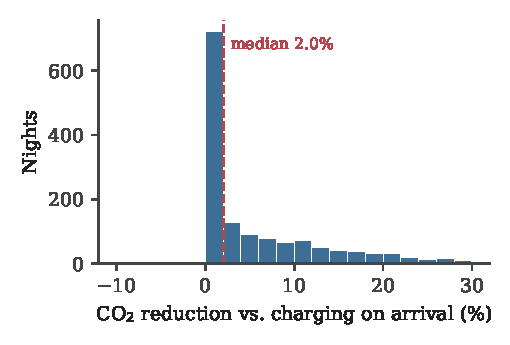
\includegraphics[width=\columnwidth]{figures/backtest_distribution.pdf}
\caption{Distribution of nightly CO$_2$ reduction vs.\ charging on arrival, 1,448 nights of the corrected Spanish record.}
\label{fig:backtest}
\end{figure}

Cost and carbon genuinely conflict: the cheapest and cleanest hour of a night coincide on only 18.0\% of nights, and minimizing cost leaves emissions 4.3\% above the emissions optimum while minimizing emissions leaves the bill 4.5\% above the cost optimum. A dirtier, more variable grid (Germany, mean intensity 358.4 vs.\ Spain's 254.7 gCO$_2$eq/kWh) saves \emph{less} on a typical night (median 1.0\% vs.\ 2.0\%) but more in total (8.2\% vs.\ 6.6\%), because charging on arrival already lands on Germany's cleanest hour by a wider margin ($-7.4\%$ vs.\ $-2.7\%$ below the night mean); dirtiness and variability predict the best nights, not the typical one.

\subsection{Hosting capacity, and its validation}
Table~\ref{tab:hosting} and Fig.~\ref{fig:hosting} give the headline result: on a measured 89~kW residential baseline for 200 homes, coordinating charging against a 250~kW transformer raises hosting capacity from 75 vehicles (on arrival) to a median 308 (coordinated) over 20 fleet draws -- a 4.1$\times$ gain. The full range across draws is 3.3--5.3$\times$, but a range over 20 samples is not a confidence interval: bootstrap-resampling those same 20 draws (10,000 resamples, percentile method) gives a much tighter 95\% CI of [3.73$\times$, 4.24$\times$], since the range's extremes come from one or two unusually favourable or unfavourable fleet seeds rather than typical sampling variation. The mechanism is that the binding constraint moves from instantaneous power (charging on arrival fills one or two hours of a thirteen-hour window) to energy (coordination spreads the same load across the whole window). The gain is largest on the tightest transformer (5.8$\times$ at 160~kW) and smallest on the loosest (3.7$\times$ at 630~kW); Table~\ref{tab:hosting}'s other ratings rest on only 6 draws each, so their intervals are correspondingly wider.
\begin{table}[t]
\centering
\caption{Hosting capacity by transformer rating (median over fleet draws, with a bootstrap 95\% CI on the gain).}
\label{tab:hosting}
\begin{tabular}{lrrrr}
\toprule
\textbf{Rating} & \textbf{Arrival} & \textbf{Coord.} & \textbf{Gain} & \textbf{95\% CI} \\
\midrule
160 kW & 25 & 148 & 5.8$\times$ & [4.33, 6.84] \\
250 kW & 75 & 308 & 4.1$\times$ & [3.73, 4.24] \\
400 kW & 151 & 580 & 3.8$\times$ & [3.41, 4.28] \\
630 kW & 272 & 990 & 3.7$\times$ & [3.35, 3.84] \\
\bottomrule
\end{tabular}
\end{table}
\begin{figure}[t]
\centering
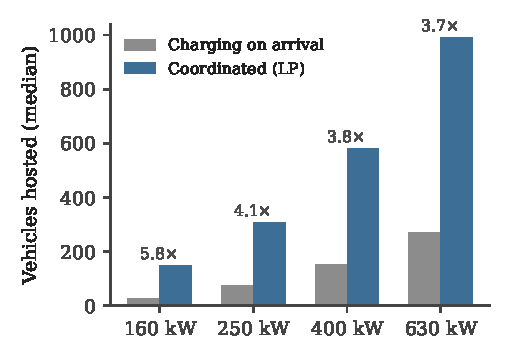
\includegraphics[width=\columnwidth]{figures/hosting_capacity.pdf}
\caption{Hosting capacity vs.\ transformer rating: charging on arrival vs.\ coordinated.}
\label{fig:hosting}
\end{figure}

This headline survives a one-at-a-time sensitivity sweep over baseline peakiness, arrival/departure behavior, energy per vehicle, charger mix, and homes per transformer: no single varied input pushes the gain below 5.0$\times$, and a peakier baseline \emph{raises} it to 7.8--10.2$\times$. It also survives validation against real household panels (Table~\ref{tab:validation}): on Spain's GoiEner panel the real-street gain (4.9--5.0$\times$) sits inside the model's own fleet-draw noise band; on the UK's Low Carbon London panel, whose households peak later and more sharply, coordination is worth roughly twice as much (10.0--10.7$\times$) -- the direction the sensitivity sweep already predicted for a peakier baseline.
\begin{table}[t]
\centering
\caption{Hosting-capacity gain, modeled vs.\ real household panels.}
\label{tab:validation}
\begin{tabular}{lrr}
\toprule
\textbf{Region (evidence)} & \textbf{Modeled gain} & \textbf{Real-street gain} \\
\midrule
Spain (GoiEner panel~\cite{quesada2024goiener}) & 5.3$\times$ & 4.9--5.0$\times$ \\
UK (Low Carbon London~\cite{tindemans2023lcl}) & 5.3$\times$ & 10.0--10.7$\times$ \\
India (published figure only) & 3.5$\times$ & 3.2--3.3$\times$ \\
\bottomrule
\end{tabular}
\end{table}

\subsection{Forecast robustness: a day-ahead model and a decision gate}
A ridge forecaster trained on the 2024 Spanish grid and scored, unseen, on 2025 reaches a mean absolute error of 15.6~gCO$_2$/kWh and captures 80.9\% of the achievable saving on the modern (higher-solar) grid, against 68.9\% on the older, less predictable 2018 grid. Per-night behavior is uneven: on nights with real structure the forecast captures 92--98\% of the achievable saving, but on nearly flat nights forecast error exceeds the spread being chased, and scheduling on it does worse than charging on arrival -- 10 of 46 served 2018 nights and 10\% of 2025 nights.

A decision gate that computes, at commitment time, the saving the forecast \emph{expects} and defers to charging on arrival below a threshold $\tau$ fixes most of this (Fig.~\ref{fig:gate}): at $\tau=4\%$, 47\% of nights are acted on, the fleet-total saving \emph{rises} slightly to 5.74\% (73.6\% of the oracle), and the share of nights worse than charging on arrival falls from 26.6\% to 7.8\%. The gate is a safety measure, not a free lunch: pushed too high ($\tau=15\%$) it discards 55\% of the oracle's saving to avoid a residual 1.1\% of harmful nights.
\begin{figure}[t]
\centering
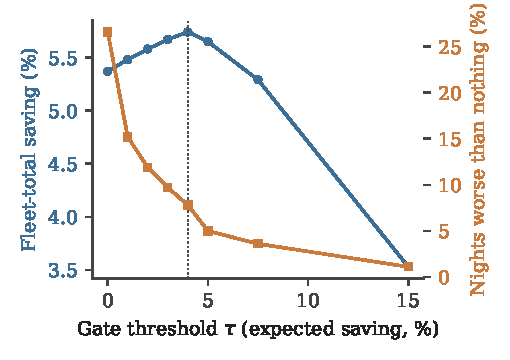
\includegraphics[width=\columnwidth]{figures/forecast_gate.pdf}
\caption{Forecast-gate sweep, Spain, 361 held-out nights: fleet-total saving and share of nights worse than charging on arrival, by gate threshold $\tau$.}
\label{fig:gate}
\end{figure}

\subsection{Rolling-horizon control loses to the one-shot plan}
Rebuilding the carbon scheduler as an hourly re-solving MPC controller and replaying it over 362 held-out nights \emph{raises} mean regret against perfect foresight from 2.521\% (one-shot LP) to 2.965\% -- 18\% relatively worse, better on 96 nights, worse on 124. Decomposing the loss: committing hour-by-hour instead of all at once costs essentially nothing ($-0.022$ percentage points), while refreshing the forecast every hour costs $+0.465$ points -- better information, used this way, makes the schedule worse. A deferral penalty intended to discourage over-optimistic waiting was swept from 0 to 2$\times$ the forecast's own horizon-dependent error and made regret rise monotonically at every strength tested (2.965\% to 3.945\%), closing that repair for this formulation.

\subsection{India: a different fleet, and a different answer}
India's EV registrations are 56\% two-wheelers, 35\% three-wheelers, and only 8\% cars~\cite{fada2025}, against a European model's implicit assumption of cars throughout. Per 100 vehicles the Indian mix wants 2.3$\times$ less energy and 4.9$\times$ less connected power than an equivalent European fleet. Re-deriving hosting capacity for this mix on a 100~kVA, 150-home Indian distribution transformer gives 35 vehicles on arrival against 123 coordinated -- a 3.5$\times$ gain, the same order as Spain's, because the underlying mechanism (instantaneous power vs.\ energy) does not depend on vehicle class. Capacity is also seasonal: the same transformer hosts 143 vehicles in winter and 107 in summer, because summer's air-conditioning load is both higher overnight and flatter across the window, removing the valley coordination exploits.

Carbon tells the opposite story. India's measured grid runs at 592~gCO$_2$eq/kWh, 2.3$\times$ Spain's, but overnight carbon-aware charging there saves a median of only 0.09\% -- about 22$\times$ smaller than Spain's 2.0\%, because the overnight window sits almost flat at India's dirtiest hours (peaking near 03:00--05:00) while the grid's actual clean period is midday solar, outside the charging window entirely. Where a saving exists, it is in a daytime charging window (median 1.51\%), which is a workplace or depot's problem, not an overnight residential one. In the full simulator scenario, coordinating an 80-vehicle Indian fleet against a 60~kW feeder cuts peak load 71.1\% and leaves carbon essentially untouched (0.0\% on the median night) -- the capacity result, not the carbon one, is what India's grid rewards.

\subsection{Robustness of the capacity gain to forecast error}
Finding 10's 123-vehicle Indian capacity figure assumes perfect knowledge of the street's other demand at the moment the schedule is committed. Holding back a feeder margin $m$ as insurance against error already costs capacity even under a perfect forecast: capacity falls from 123 ($m=0$) to 37 ($m=30\%$) -- by a 30\% margin coordination has given back nearly all of its own gain. A first, coarse sweep of $m$ at the national day-ahead demand forecaster's own measured error ($\sigma=3\%$, the AR(1) model of \eqref{eq:ar1}) over 6 margins and 60 draws each reported its best case as 35\% overload at $m=20\%$. A 6-point grid cannot rule out a better margin between grid points, and 60 draws gives no formal uncertainty bound on that number, so we re-ran the same error level on an 11-point grid (every 4 points, 0--40\%) with 100 draws per margin and a bootstrap 95\% CI (10,000 resamples) at each point. The finer grid finds a \emph{better} margin than the coarse one did: $m=28\%$, not 20\%, gives the lowest overload probability on the grid, 25.0\% (95\% CI [17\%, 34\%]) at a capacity of 42 vehicles -- still more than 3$\times$ the 5\% target even at the most favourable edge of its own confidence interval, and no margin on the 11-point grid meets the target at its 95\% CI upper bound. Margins of 36\% and above collapse capacity to 0: at that point the de-rated limit sits at or below what the houses alone draw on an unlucky forecast draw, so scheduling fails before a single vehicle is added.

Finding 23 left open whether a controller that re-forecasts every hour rather than committing once to a margin could buy back this reliability. Algorithm~\ref{alg:rolling}'s rolling controller answers no: Fig.~\ref{fig:intraday} and Table~\ref{tab:intraday} show that in 8 of the 12 error-bearing cells tested, rolling control overloads \emph{more} often than the static one-shot plan, by a mean 15.0 percentage points and a worst case of 33.4 points; the 2 cells that favor rolling are within one draw out of thirty of the static result and occur where static control is already failing on every draw. At zero error both controllers agree exactly, which is the same time-consistency check used elsewhere in this project, confirming the degradation is a property of forecasting under commitment and not an artifact of the rolling implementation.
\begin{figure}[t]
\centering
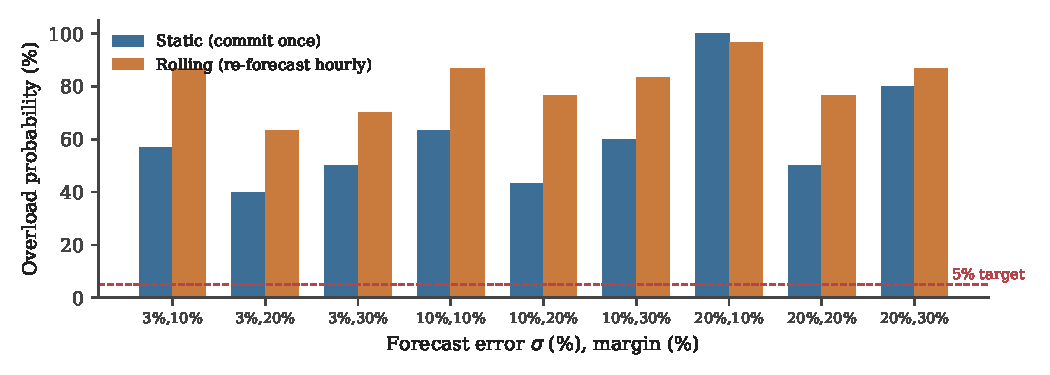
\includegraphics[width=\columnwidth]{figures/intraday_overload.pdf}
\caption{Overload probability, static (commit once) vs.\ rolling (re-forecast hourly) control, by forecast error $\sigma$ and margin, 100~kVA India transformer.}
\label{fig:intraday}
\end{figure}
\begin{table}[t]
\centering
\caption{Static vs.\ rolling overload probability, selected cells.}
\label{tab:intraday}
\begin{tabular}{rrrrr}
\toprule
$\sigma$ & \textbf{Margin} & \textbf{Static} & \textbf{Rolling} & \textbf{Diff} \\
\midrule
3\% & 10\% & 56.7\% & 86.7\% & +30.0 pp \\
3\% & 20\% & 40.0\% & 63.3\% & +23.3 pp \\
10\% & 10\% & 63.3\% & 86.7\% & +23.4 pp \\
10\% & 20\% & 43.3\% & 76.7\% & +33.4 pp \\
20\% & 20\% & 50.0\% & 76.7\% & +26.7 pp \\
20\% & 30\% & 80.0\% & 86.7\% & +6.7 pp \\
\bottomrule
\end{tabular}
\end{table}

The mechanism is the same one identified for carbon MPC (Section~\ref{sec:experiments}E) in a different problem: a static controller sees one (possibly wrong) forecast for the whole night and spreads its single mistake flat across thirteen hours; a rolling controller commits hour-by-hour against a belief that keeps changing, so a correction that arrives late in the night has to be absorbed by whatever flexibility is left, which is the least flexibility of the whole window. Two implementation defects produced this same symptom before being caught and fixed (Section~\ref{sec:discussion}), which is reported here because a result this close to the earlier bugs' own symptom needed an independent check before it could be trusted.

\section{Discussion}
\label{sec:discussion}

Two results in this paper -- carbon MPC (Section~\ref{sec:experiments}E) and the intraday hosting-capacity controller (Section~\ref{sec:experiments}G) -- reach the same qualitative conclusion by independent routes: giving a committed scheduler better information \emph{as it goes}, rather than a single forecast up front, does not reliably help, because early commitments consume exactly the flexibility a late correction would need. This is not an argument that forecasting is worthless -- the day-ahead forecaster captures up to 81\% of achievable carbon saving, and forecast quality improves monotonically with proximity to real time (MAE 4.96~g at one hour ahead to 20.49~g at thirteen). It is an argument that \emph{how} a controller consumes improving information matters as much as the information's quality, and that the naive expectation -- waiting for better data should pay for itself -- needs to be measured, not assumed, for a given formulation.

Two implementation defects in the intraday controller are worth naming because a run that had quietly shipped either would have reported the same qualitative result (rolling control loses) for the wrong reason. First, the shared scheduler used elsewhere in this project returns only a fleet's \emph{summed} hourly load; handed to a per-vehicle-group energy tracker, that summed value was credited to every group separately, overcommitting a single hour by roughly 10$\times$. Second, re-solving repeatedly against a flat-objective LP let the solver pick a different arbitrary tied solution at each re-solve, compounding into a last-minute energy crunch unrelated to forecast error; minimizing peak load removed the degeneracy. Both were caught by the same check -- a zero-error run must reproduce the static optimum exactly -- which is why that check is reported as part of the method (Section~\ref{sec:method}D) rather than treated as incidental testing.

The hosting-capacity headline itself survived three corrections during this project (an unstaggered-arrival assumption that inflated it 2.7$\times$, a sevenfold-overstated residential baseline, and a bisection search that once reported its own numerical bound as a ceiling), and the smart-meter validation in Section~\ref{sec:experiments}D was explicitly designed to catch a fourth kind of error -- a wrong \emph{shape} assumption for household demand -- rather than to produce a tighter confidence interval. That it landed inside the model's own sensitivity band for Spain, and in the direction the sensitivity sweep predicted for the UK's peakier households, is evidence the mechanism is right even where the inputs were not.

\section{Limitations and Future Work}
\label{sec:limitations}

The residential baseline for the headline hosting-capacity figure is system-wide load scaled to a street, not a metered feeder; the smart-meter validation (Section~\ref{sec:experiments}D) addresses the baseline's \emph{shape} but not the fleet assumptions (arrival-time and energy-per-vehicle distributions), which remain a sensitivity sweep rather than a measurement. Session-level charging data such as ACN-Data~\cite{leeacndata} would close this gap, but it is not a bare download: we confirmed directly that its API returns HTTP 401 (``please provide proper credentials'') without an access token, and that obtaining one requires registering a real name, institutional affiliation, and job role, not an automated request -- access is gated on the account holder, not on us. GridSense schedules against \emph{average} carbon intensity derived from measured generation mix; load shifting responds to the \emph{marginal} generator, and closing that gap needs marginal operating emissions rate (MOER) data this project does not have~\cite{watttime_moer}. India's illustrative time-of-day price in the simulator rests on a reported tariff shape~\cite{ceew2025tariff,merc2025} rather than a verified published schedule, and is labeled as such rather than measured. The intraday controller's forecast-error levels beyond the national day-ahead figure (3\%) are guessed brackets, not measured feeder-level error, and its margin is held fixed through the night; a margin that itself narrows as uncertainty resolves, or a correction model that can learn a systematic (rather than purely mean-reverting) bias, remain untested. The rolling-vs-static comparison (Section~\ref{sec:experiments}G) and the carbon MPC comparison (Section~\ref{sec:experiments}E) are both measured only against this project's own one-shot LP, not against a published alternative controller (a scenario-based robust formulation, or a reinforcement-learning scheduler) -- a head-to-head against prior work's own methods, not just an internal ablation, remains open. Finally, every result here comes from a single LP formulation and a single solver; whether the rolling-control loss is intrinsic to forecasting-under-commitment in general, or an artifact of this particular objective and re-solve cadence, is a question a different controller family could still answer differently.

\section{Conclusion}
\label{sec:conclusion}

Measured against real grid data rather than synthetic assumptions, coordinated EV charging's value is unevenly distributed across the three things it is usually sold on. Carbon savings are real but modest and long-tailed. Distribution hosting capacity is where the economically significant number lives, and it is the one result that transfers intact to a market -- India -- whose vehicle mix, grid, and carbon mechanism are otherwise entirely different from the European case this project started from. Forecast robustness is the least settled: a day-ahead forecaster and a decision gate recover most of carbon-aware scheduling's value, but two independent experiments, on two different objectives, show that re-forecasting more often under commitment is not automatically an improvement, and can reliably be worse. Every headline figure in this paper has been wrong at least once during its own development; reporting those corrections alongside the current numbers is, we think, part of what makes a measurement-driven claim worth trusting.

\appendix
Table~\ref{tab:repro} maps each reported result to the script that reproduces it.
\begin{table}[h]
\centering
\caption{Reproducibility.}
\label{tab:repro}
\begin{tabular}{p{3.0cm}p{4.8cm}}
\toprule
\textbf{Script} & \textbf{Reproduces} \\
\midrule
\texttt{export\_evidence.py} & Coupling-constraint table (\S\ref{sec:experiments}A) \\
\texttt{backtest.py} & Nightly saving distribution (\S\ref{sec:experiments}B) \\
\texttt{train.py}, \texttt{train\_v2.py} & Synthetic-curve inversion, deployed ridge forecaster \\
\texttt{export\_hosting\_capacity.py} & Hosting-capacity table and figure (\S\ref{sec:experiments}C) \\
\texttt{bootstrap\_hosting.py} & Hosting-capacity gain bootstrap CI (\S\ref{sec:experiments}C) \\
\texttt{sensitivity\_hosting.py} & One-at-a-time hosting sensitivity sweep \\
\texttt{validation/} & Smart-meter validation (\S\ref{sec:experiments}C) \\
\texttt{spread\_gate.py} & Forecast-gate sweep and figure (\S\ref{sec:experiments}D) \\
\texttt{train\_horizon.py}, \texttt{mpc.py} & Rolling-horizon MPC result (\S\ref{sec:experiments}E) \\
\texttt{india\_fleet.py}, \texttt{export\_india\_capacity.py} & Indian fleet and hosting capacity (\S\ref{sec:experiments}F) \\
\texttt{india\_carbon.py}, \texttt{india\_backtest.py} & Indian carbon-saving result \\
\texttt{india\_robustness.py} & Margin-vs-error overload table (\S\ref{sec:experiments}G) \\
\texttt{india\_margin\_search.py} & Fine-grained margin search and bootstrap CI (\S\ref{sec:experiments}G) \\
\texttt{india\_robustness\_intraday.py} & Static-vs-rolling overload figure and table (\S\ref{sec:experiments}G) \\
\bottomrule
\end{tabular}
\end{table}

\section*{Acknowledgment}
The authors thank the maintainers of Energy-Charts, ENTSO-E, Grid-India, GoiEner, and the Low Carbon London project for the open, measured data this work depends on.

\begin{thebibliography}{17}

\bibitem{kakkar2024}
R. Kakkar, S. Agrawal, and S. Tanwar, ``A systematic survey on demand response management schemes for electric vehicles,'' \emph{Renewable and Sustainable Energy Reviews}, vol. 203, 2024.

\bibitem{golgol2024}
M. Golgol, A. Pal, V. Vittal, C. Fini, E. Palomino, and K. Girardi, ``Exploring the Influence of Residential Electric Vehicle Charging on Distribution System Hosting Capacity -- A Case-Study in Arizona,'' \emph{arXiv preprint arXiv:2411.09990}, 2024.

\bibitem{paudyal2021}
P. Paudyal, S. Ghosh, S. Veda, D. Tiwari, and J. Desai, ``EV Hosting Capacity Analysis on Distribution Grids,'' National Renewable Energy Laboratory, NREL/CP-5D00-75639, 2021.

\bibitem{yang2020bmpc}
L. Yang, X. Geng, X. Guan, and L. Tong, ``Deferrable Load Scheduling under Demand Charge: A Block Model-Predictive Control Approach,'' \emph{arXiv preprint arXiv:2012.14624}, 2020.

\bibitem{lago2021}
J. Lago, G. Marcjasz, B. De Schutter, and R. Weron, ``Forecasting day-ahead electricity prices: A review of state-of-the-art algorithms, best practices and an open-access benchmark,'' \emph{Applied Energy}, vol. 293, 2021.

\bibitem{uniejewski2024}
B. Uniejewski, ``Regularization for electricity price forecasting,'' \emph{Operations Research and Decisions}, vol. 34, no. 3, pp. 267--286, 2024.

\bibitem{gandhi2021v2g}
H. A. Gandhi and A. D. White, ``City-wide modeling of Vehicle-to-Grid Economics to Understand Effects of Battery Performance,'' \emph{arXiv preprint arXiv:2108.05837}, 2021.

\bibitem{radovanovic2021}
A. Radovanovi{\'c} \emph{et al.}, ``Carbon-Aware Computing for Datacenters,'' \emph{arXiv preprint arXiv:2106.11750}, 2021.

\bibitem{watttime_moer}
WattTime, ``MOER Modeling,'' technical white paper, 2022. [Online]. Available: https://watttime.org/wp-content/uploads/2023/11/WattTime-MOER-modeling-20221004.pdf

\bibitem{ipcc2014ar5}
IPCC, ``Annex III: Technology-specific cost and performance parameters,'' in \emph{Climate Change 2014: Mitigation of Climate Change. Contribution of Working Group III to the Fifth Assessment Report of the Intergovernmental Panel on Climate Change}. Cambridge, U.K.: Cambridge Univ. Press, 2014.

\bibitem{ree_pvpc}
Red El\'ectrica de Espa\~na and Ministerio para la Transici\'on Ecol\'ogica (MITECO), ``Precio Voluntario para el Peque\~no Consumidor (PVPC).'' [Online]. Available: https://www.ree.es/en/operation/electricity-system/pvpc

\bibitem{quesada2024goiener}
C. Quesada, L. Astigarraga, C. Merveille, and C. E. Borges, ``An electricity smart meter dataset of Spanish households: insights into consumption patterns,'' \emph{Scientific Data}, vol. 11, art. 59, 2024.

\bibitem{tindemans2023lcl}
S. Tindemans, ``Low Carbon London smart meter data (refactored),'' 4TU.ResearchData, 2023. doi: 10.4121/fbbe775b-48d8-469f-a39b-b64488bfd6fd.

\bibitem{fada2025}
Federation of Automobile Dealers Associations (FADA), India, EV retail sales data, calendar year 2025, as reported in ``EV Retail Sales Jump 16\% In 2025 On 77\% Surge In Electric Car Demand: FADA,'' \emph{Free Press Journal}, 2026.

\bibitem{ceew2025tariff}
Council on Energy, Environment and Water (CEEW), ``How can electricity tariff reforms empower Indian households?,'' CEEW blog, 2025.

\bibitem{merc2025}
Maharashtra Electricity Regulatory Commission (MERC), Press Note on Multi-Year Tariff Order for Tata Power Company -- Distribution, 2025. [Online]. Available: https://merc.gov.in

\bibitem{leeacndata}
Z. J. Lee, T. Li, and S. H. Low, ``ACN-Data: Analysis and Applications of an Open EV Charging Dataset,'' in \emph{Proc. 10th ACM Int. Conf. Future Energy Systems (e-Energy '19)}, Phoenix, AZ, USA, Jun. 2019.

\end{thebibliography}

\end{document}
